\section{Reflection}
\subsection{Perspective}
Although our web site was improved greatly, but the amelioration is always existing.
\begin{enumerate}
\item{Security}
The security is always the most important thing to do. Several actions could be adopted.
\begin{itemize}
\item{HTTPS Protocol}
Foe the users' sign in and sign up pages, they should be applied the HTTPS protocol to provide a white list to avoid attackers.
\item{Robots Exclusion Protocol}
Robots exclusion protocol is used to define what we want to be quoted by the search engine (like google, yahoo). Some admin parts of the web site and also some private data do not hope to be published into the internet, then we can define the contents what we hope not to be visited by the search engine in robot.txt, and put this file into the Rails.root path. 
\begin{figure}[h!]
    \centering
    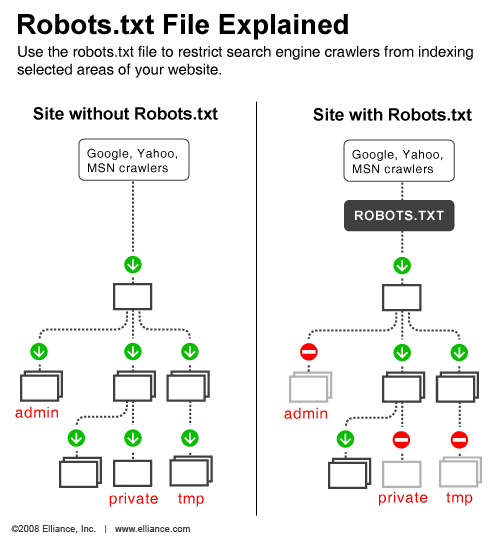
\includegraphics[width=12cm]{robot.jpg}
    \caption{All function-oriented branches }
    \label{fig-sample}
\end{figure} 
\end{itemize} 
\end{enumerate}
\subsection{Industrial analyse}
After WRSC, occasionally discussed with some Finnish engineers, we found out that they had developed a similar tracking product in order to follow the trace(http://www.thingsee.com/). Comparing our tracking system with their product, they are nearly the same, except their product contains more sensors, so they can measure more parameters, like: temperature, motion and so on, and the price of product is more than 300 Euros. Although our tracking system do not have so much sensors, but it cost much less than their product, the price of our tracking system is less than 100 Euros.
Furthermore, we found another similar project from the internet, in Brittany, France.(https://www.gwenneg.bzh/fr/tifiz) So it was not impossible to develop our own product in the near future.
\subsection{Personal analyse}
I am glad to have such a good opportunity to take part in a passionate project and also I am glad to be in Aland, Finland for my internship where I discovered a beautiful place with friendly awesome people. This impressive experience not only reinforces what I had learned, but also permit me to discover the world, to learn how real engineers realize their aims and especially work professionally under pressures.